\documentclass{beamer}
\input{config/rc-slides-config.tex}
\usepackage[english]{babel}
\usepackage{amsfonts}
\usepackage{amsmath}
\usepackage{amssymb}
%\usepackage{subfig}
\usepackage{graphicx}
\usepackage{array}
\usepackage{natbib}
%\usepackage{caption}
% \usepackage{mathtools}
% \usepackage{algorithm}
% \usepackage{algorithmic}
%\usepackage{tabularx}
%\usepackage{xltabular}  
%\usepackage{booktabs} 
\usepackage{xcolor}
\usepackage{makecell}
\usepackage{lipsum}
% \usepackage{tikz} 
%\usepackage{minted}
% \usepackage{setspace}
\usepackage{hyperref}

\begin{document}
	
\title[Secondary patterns]{Secondary patterns in basic models of opinion dynamics}
\institute[UV]{\textbf{Instituto de Investigaciones en Inteligencia Artificial} \\ Universidad Veracruzana \\ \vspace{0.25cm} \emph{Campus Sur, Calle Paseo Lote II, Sección Segunda No 112, \\ Nuevo Xalapa, Xalapa, Ver., México 91097}  \\ 
	\vspace{0.25cm}   
}
\author[Ulises J. G.]{Ulises Jiménez Guerrero}
\date[MIA 2026]{\today}

\logo{
	
\includegraphics[width=0.8cm]{figs/logo_UV.png} 
}


\begin{frame}
	\maketitle
\end{frame}

\section{Secondary patterns}

\subsection{Searching for secondary patterns}
\begin{frame}{Secondary patterns}
	\begin{itemize}
		\item The model was able to approximate the main pattern:opinion share over three time steps and the election results. However, following POM, we need to evaluate it's capacity to reproduce secondary patterns.
		\item The secondary pattern that will be evaluated is the vote share for option A by gender: male and female.
		\item Given that this was not reported, the data must be extracted from the database. 
	\end{itemize}
\end{frame}

\begin{frame}{Adjusting the model}
	\begin{itemize}
		\item From the 1070 observations in the first poll, only the subjects with preference for the main options were selected. After this, there were only 858 observations left. 
		\item The model was adapted, adding a new variable for age to each patch. These are read from the first poll.
		\item The preference share by gender for option A was calculated at the time of the third poll. It was found that the value was $60\%$ for both genders. That is, 60\% of all men in the third poll had a preference for option A, same for women.
	\end{itemize}
\end{frame}

\begin{frame}{Secondary patterns in the positive influence model}
	\begin{itemize}
		\item The positive influence model was used to evaluate secondary patterns.
		\item Keeping the optimal parameters found in the previous experiments, 30 runs were tried to find the preference share for A at the time of the third poll for men and women.
		\item \textbf{The model wasn't able to reproduce the secondary pattern for neither gender}, with a simulated value higher than the reported in the poll.
	\end{itemize}
\end{frame}

\begin{frame}{Male preference share for A}
	\begin{figure}[h!]
		\centering
		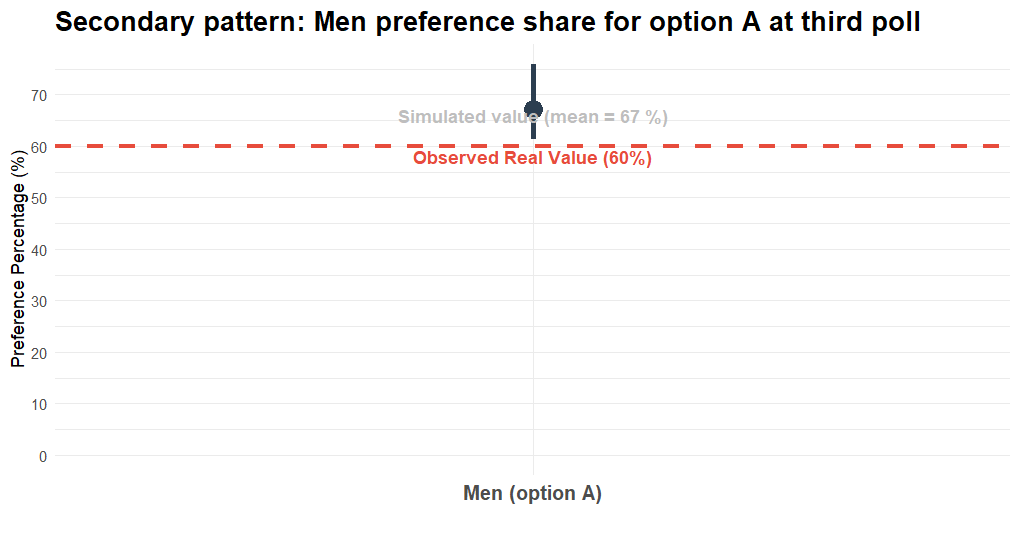
\includegraphics[width=1\linewidth]{figs/secundario_hombre_V2}
	\end{figure}
\end{frame}

\begin{frame}{Female preference share for A}
	\begin{figure}[h!]
		\centering
		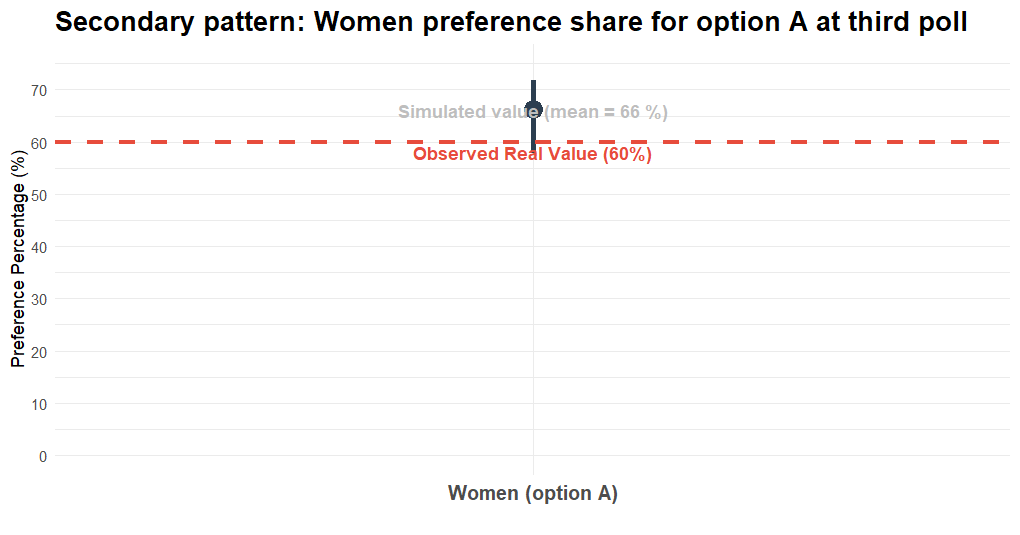
\includegraphics[width=1\linewidth]{figs/secundario_mujeres_V2}
	\end{figure}
\end{frame}

\begin{frame}{Adjusting model and searching for patterns}
	\begin{itemize}
		\item Given the changes made to the model, it was adjusted to find new optimal parameters. Following the methodology used in the previous section, these new optimal values were found to be \textit{learning-rate = 0.71}, \textit{agents-updated-per-tick = 5}. 
		
		\item The model was tried once again for its capacity to reproduce vote share for A by gender. It gave similar results, with a share of 65\% for both genders. However, the variability in the results slightly decreased.
	\end{itemize}
\end{frame}


\begin{frame}{Male preference share for A for adjusted model}
	\begin{figure}[h!]
		\centering
		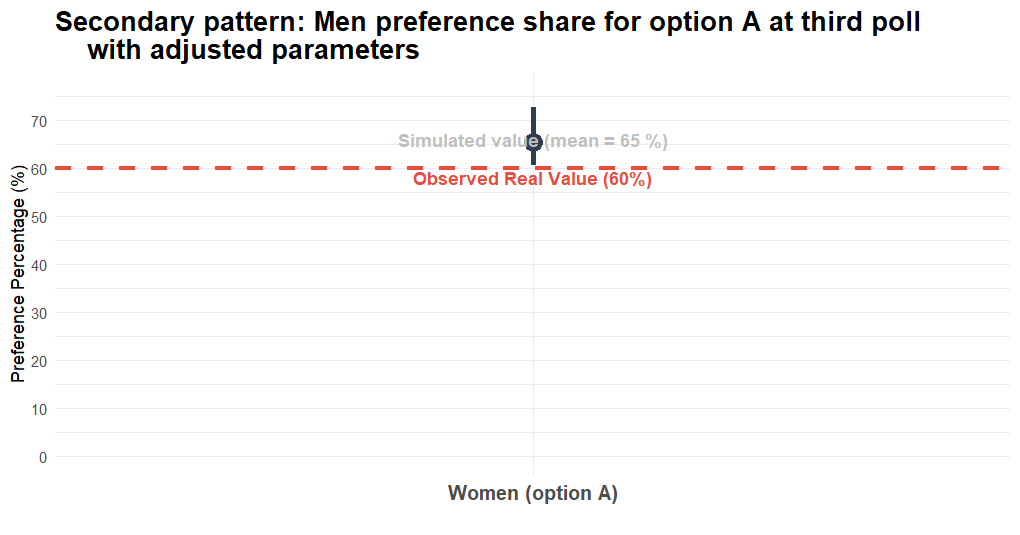
\includegraphics[width=1\linewidth]{figs/secundario_ajustado_hombres_V2.png}
	\end{figure}	
\end{frame}

\begin{frame}{Female preference share for A for adjusted model}
	\begin{figure}[h!]
		\centering
		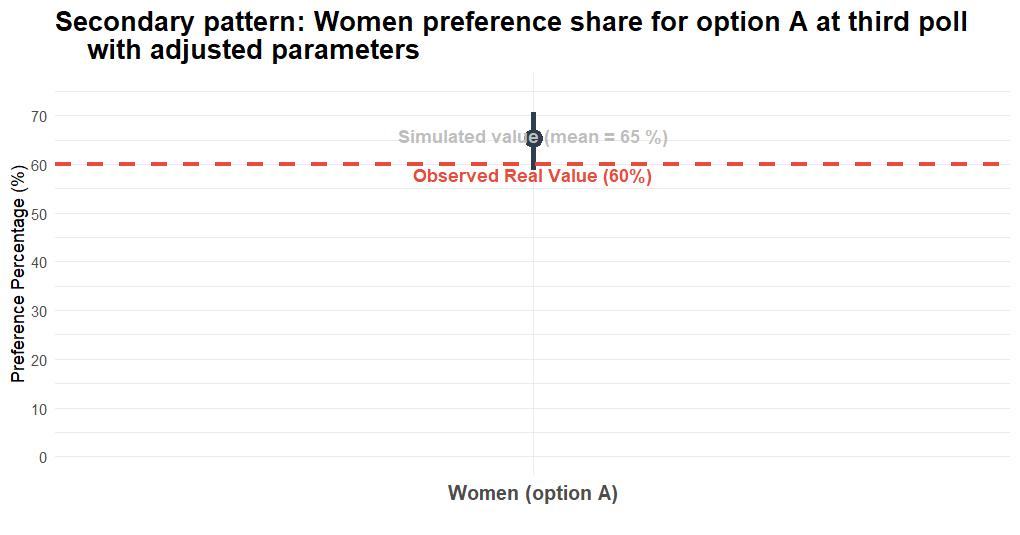
\includegraphics[width=1\linewidth]{figs/secundario_ajustado_mujeres_V2.png}
	\end{figure}	
\end{frame}

\subsection{Taking opinions from poll}
\begin{frame}{Using opinions from poll}
	\begin{itemize}
		\item Given the model's failure to reproduce the secondary pattern of preference share per gender, a last experiment was tried taking the opinion directly from the poll.
		\item Based on the database, each agent was given a random preference for option A or B with values between 0 and 1, with an uniform distribution.
		\item The model was modified to reflect this, having a final third version.
	\end{itemize}
\end{frame}

\begin{frame}{Secondary patterns taking opinions from poll}
	\begin{itemize}
		\item Firstly, the model was tried for secondary patterns using the best values for the parameters found in the initial section. It gave an even worse performance than the previous version, with a higher error in relationship to the preference share by gender, with a mean of 74\% for men and 75\% for women. 
		\item New optimal parameters were found for the model, with \textit{learning-rate = 0.17} and \textit{agents-updated-per-tick = 1}. The mean preference share for option A was found to be 65\% for men, 68\% for women. These results are very similar to the previous model, with a very limited variability. 
	\end{itemize}
\end{frame}

\begin{frame}{Male preference for A taking opinions from poll}
	\begin{figure}[h!]
		\centering
		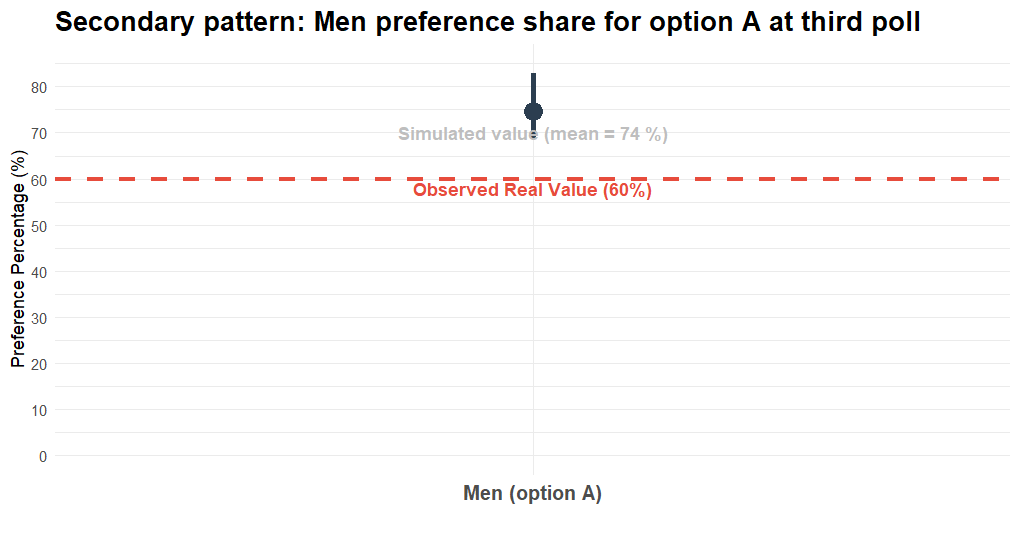
\includegraphics[width=1\linewidth]{figs/secundario_hombre_V3}
	\end{figure}
\end{frame}

\begin{frame}{Female preference for A taking opinions from poll}
	\begin{figure}[h!]
		\centering
		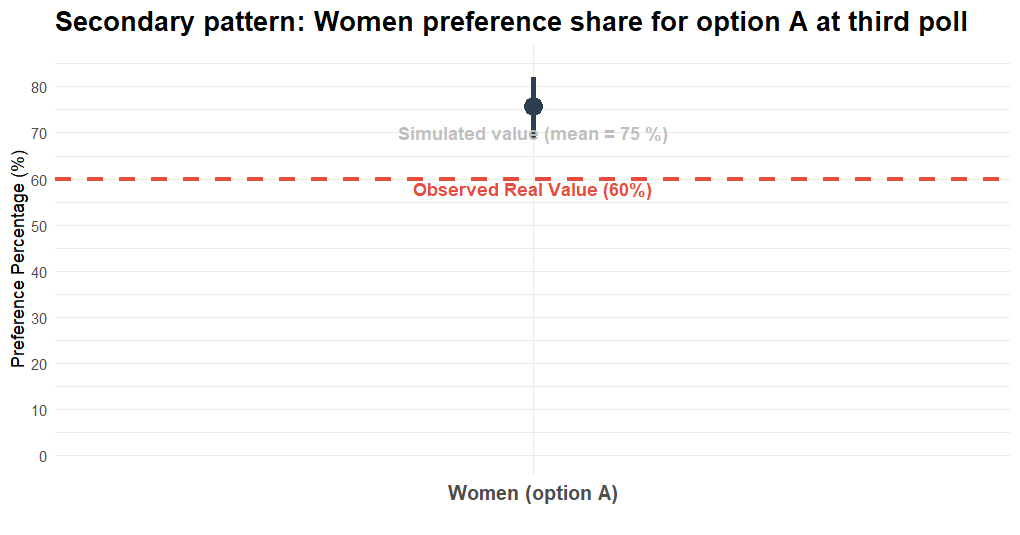
\includegraphics[width=1\linewidth]{figs/secundario_mujeres_V3}
	\end{figure}
\end{frame}

\begin{frame}{Male preference for A taking opinions from poll and adjusting model}
	\begin{figure}[h!]
		\centering
		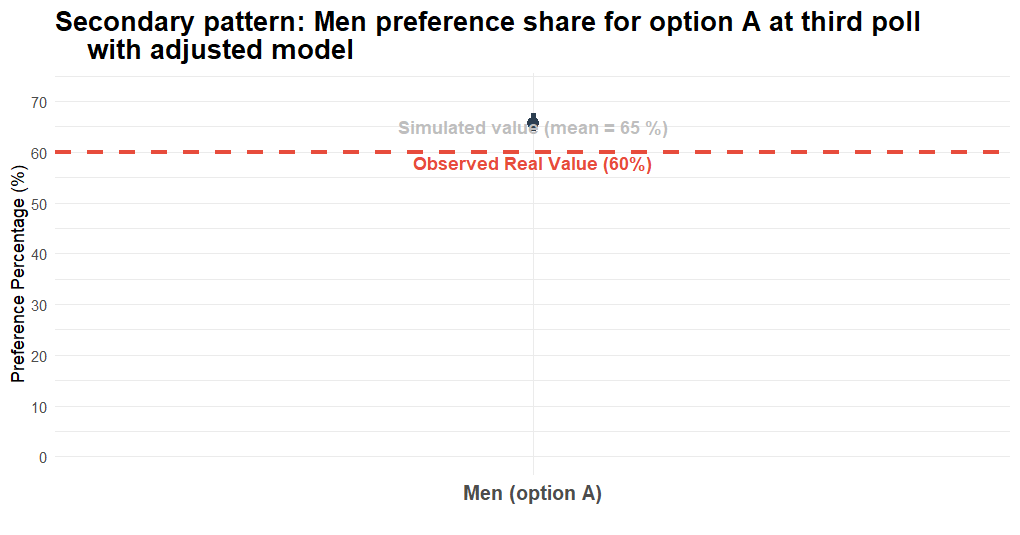
\includegraphics[width=1\linewidth]{figs/secundario_ajustado_hombres_V3}
	\end{figure}
\end{frame}

\begin{frame}{Female preference for A taking opinions from poll and adjusting model}
	\begin{figure}[h!]
		\centering
		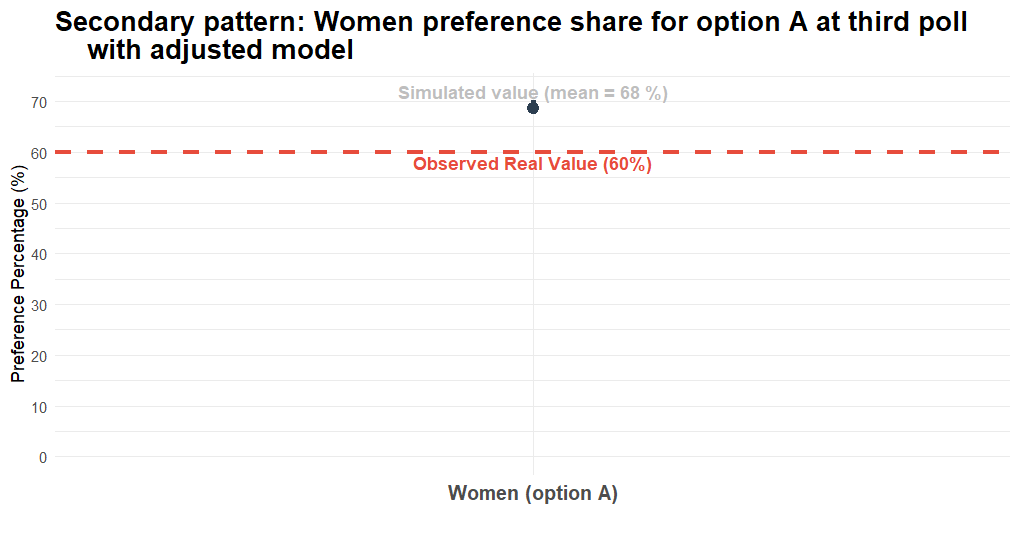
\includegraphics[width=1\linewidth]{figs/secundario_ajustado_mujeres_V3}
	\end{figure}
\end{frame}

\begin{frame}{Conclusions}
	\begin{itemize}
		\item The three types of influence modeled have the capability of providing a rough approximation to the considered three points during the election chosen as a case study.
		\item However, they lack the ability to reproduce secondary patterns such as the voter share per gender, given that the agent's characteristics aren't taken into account during the interaction.
		\item A more robust version of the model \emph{needs to take into account the characteristics of the agents at the time of interaction.} Such a model is found in Axelrod's cultural evolution model.
		\item The use of opinion polls need to be more careful, using the correct statistical methods to adjust the data. 
	\end{itemize}
\end{frame}


\end{document}